\section{Punto de Vista de Implementación Migración}

El punto de vista de implementación y migración se utiliza para relacionar programas y proyectos con las partes de la arquitectura que implementan.  Esta vista permite modelar el alcance de los programas, proyectos, actividades del proyecto en términos de las mesetas que se realizan o la arquitectura individual elementos que se ven afectados.  Además, la forma en que se ven afectados los elementos puede indicarse mediante anotando las relaciones.
Además, este punto de vista se puede utilizar en combinación con los programas y proyectos
punto de vista para apoyar la gestión de la cartera:
El punto de vista de programas y proyectos es adecuado para relacionar los objetivos comerciales con los programas y
proyectos.  Por ejemplo, esto permite analizar a un alto nivel si todos
los objetivos comerciales están suficientemente cubiertos por la (s) cartera (s) actual (es).
El punto de vista de implementación y migración es adecuado para relacionar los objetivos comerciales (y
requisitos) a través de programas y proyectos a (partes de) la arquitectura.  Por ejemplo, este
permite analizar el solapamiento potencial entre las actividades del proyecto o analizar la coherencia entre las dependencias del proyecto y las dependencias entre mesetas o
elementos de arquitectura.

\subsection{Modelo de Implementación}
\begin{figure}[h!]
	\centering
	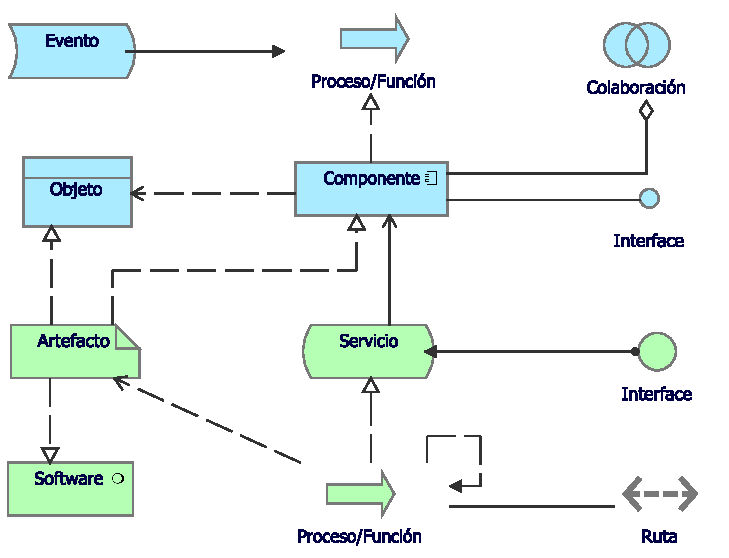
\includegraphics[width=.7\linewidth]{imgs/modelo/Implementacion.pdf}
	\caption{Modelo Implementación}
\end{figure}

El modelo de implementación y migración plasma lo referente a un resumen de los modelos de la capa de proyecto, dando lugar al reflejo total de la transición de la arquitectura actual existente a una nueva arquitectura a la que se desea llegar. Relaciona el modelo de proyecto con el modelo de migración, en donde el liberable generado como fin del paquete de trabajo se vincula o se enlaza con la primer meseta del modelo de migración.

\subsection{Caso  de Implementación}
\begin{figure}[h!]
	\centering
	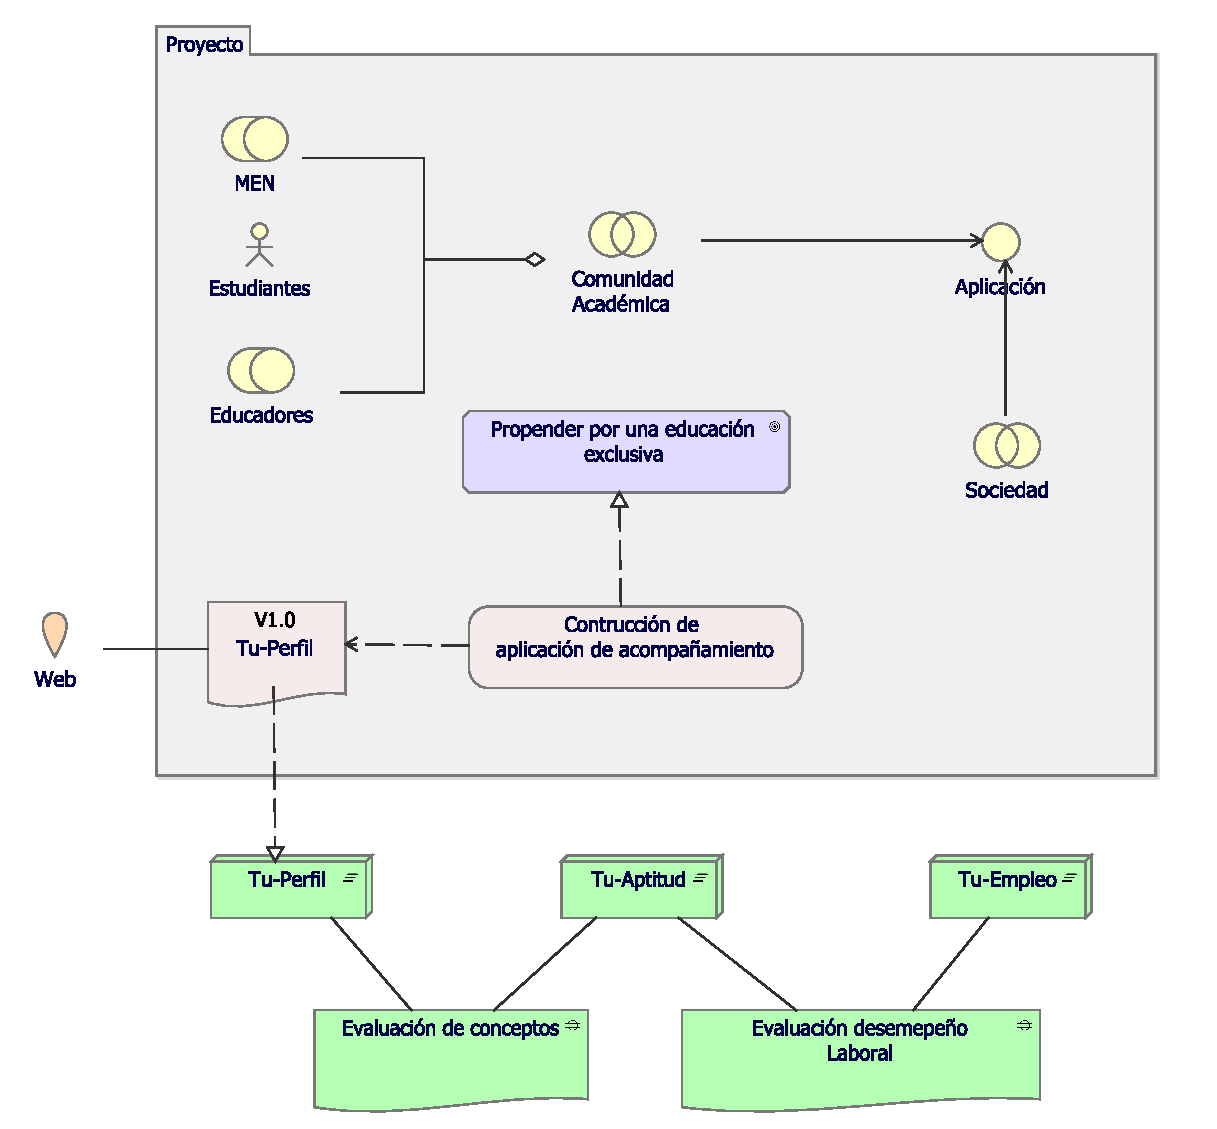
\includegraphics[width=.9\linewidth]{imgs/caso/proyecto/implementacion_migracion.pdf}
	\caption{Caso Implementación}
\end{figure}
El punto de vista de implementación/migración establece un resumen de la capa de implementación, en el cual se muestra lo que se trabajó en los puntos de vistas anteriores de esta capa. Pará el caso de estudio la aplicación de Tu-Perfil será desplegada en la web, que permitirá el acompañamiento y perfilamiento de los estudiantes. Los siguientes pasos de esta aplicación serán Tu-Aptitud que evaluar los conceptos del estudiante, y Tu-Empleo que evaluará el desempeño laboral.